\documentclass[
	xcolor={table},
	aspectratio=1610,
	18pt,
	hyperref={implicit}]{beamer}
\usetheme{Frankfurt}
\usefonttheme{professionalfonts}

%%%%%%%%%%%%%%%%%%%%%%%%%%%%%%%%%%%%%
% Document configuration
\usepackage[english,spanish,es-tabla]{babel}
\usepackage{ifthen}
\usepackage{ragged2e}
\usepackage{appendixnumberbeamer}
\usepackage{lastpage}	
\usepackage{multicol}
%%%%%%%%%%%%%%%%%%%%%%%%%%%%%%%%%%%%%

%%%%%%%%%%%%%%%%%%%%%%%%%%%%%%%%%%%%%
% Fonts, encoding & Color
\usepackage{fontspec}
%\usepackage{titlesec}

\usepackage[shortlabels]{enumitem}
%%%%%%%%%%%%%%%%%%%%%%%%%%%%%%%%%%%%%

%%%%%%%%%%%%%%%%%%%%%%%%%%%%%%%%%%%%%
% Math & chem

\usepackage{amsmath}
\usepackage{amsfonts}
\usepackage{siunitx}
\usepackage{xfrac}
\usepackage[
	modules={reactions,formula,redox,charges}
]{chemmacros}[2022/03/11]
%%%%%%%%%%%%%%%%%%%%%%%%%%%%%%%%%%%%%

%%%%%%%%%%%%%%%%%%%%%%%%%%%%%%%%%%%%%
% Figures & tables

\usepackage{graphicx}
\usepackage[justification=centering]{caption}
\usepackage{subcaption}
\usepackage{float}
\usepackage{wrapfig}

\usepackage{tabularray}
\UseTblrLibrary{varwidth}
\UseTblrLibrary{siunitx}
%%%%%%%%%%%%%%%%%%%%%%%%%%%%%%%%%%%%%

%%%%%%%%%%%%%%%%%%%%%%%%%%%%%%%%%%%%%
% Drawings & shapes

\usepackage{tikz}
\usetikzlibrary{
	shapes.geometric,
	positioning,
	arrows.meta,
	calc,
	patterns,
	patterns.meta,
	shadows,
	matrix
}

\usetikzlibrary{external}
\tikzexternalize

\tikzset{%
	external/system call={%
		xelatex \tikzexternalcheckshellescape --output-directory ./build -halt-on-error -interaction=batchmode -jobname "\image" "\texsource"%
	},
	/pgf/images/include external/.code={%
		\includegraphics{build/#1}%
	}
}

\usepackage[most]{tcolorbox}
\tcbuselibrary{raster}
\tcbuselibrary{breakable}
%\tcbuselibrary{external}
%\tcbset{external/prefix=Boxes/}
%\tcbEXTERNALIZE

\usepackage[edges,external]{forest}
\usepackage{chemplants}
%%%%%%%%%%%%%%%%%%%%%%%%%%%%%%%%%%%%%

%%%%%%%%%%%%%%%%%%%%%%%%%%%%%%%%%%%%%
% Bibliography, glossary & refs

%\usepackage[spanish]{cleveref}
\usepackage[
	toc,
	acronym,
	translate = true,
	nonumberlist
]{glossaries}
\usepackage{glossary-mcols}

\usepackage[
	thresholdtype=words
]{csquotes}

\usepackage[
	backend=biber,
	style=ieee,
	url=false,
	hyperref=true,
]{biblatex}

\usepackage{xurl}
%%%%%%%%%%%%%%%%%%%%%%%%%%%%%%%%%%%%%

%%%%%%%%%%%%%%%%%%%%%%%%%%%%%%%%%%%%%
% utils

\usepackage{adjustbox}
%%%%%%%%%%%%%%%%%%%%%%%%%%%%%%%%%%%%%
%%%%%%%%%%%%%%%%%%%%%%%%%%%%%%%%%%%%%
% Document info

\date{\today}
\title{Desalinización de agua por destilación solar activa empleando concentradores solares de lentes Fresnel}
\author{Eduardo Jiménez Miranda}
\institute{Unidad Profesional Interdisciplinaria en Ingeniería y Tecnologías Avanzadas}
%%%%%%%%%%%%%%%%%%%%%%%%%%%%%%%%%%%%%

%%%%%%%%%%%%%%%%%%%%%%%%%%%%%%%%%%%%%
% Language & localization

\selectlanguage{spanish}
\defaultfontfeatures{Ligatures=TeX}
\setmainfont{Times New Roman}
\decimalpoint
%%%%%%%%%%%%%%%%%%%%%%%%%%%%%%%%%%%%%

%%%%%%%%%%%%%%%%%%%%%%%%%%%%%%%%%%%%%
% Math & chem

% uncomment the line below only if fancyref is used
%\newcommand*\fancyrefrctlabelprefix{rct}
\chemsetup{
	reactions/own-counter = true
}

\sisetup{
	per-mode = fraction,
	group-separator={,}
}
%%%%%%%%%%%%%%%%%%%%%%%%%%%%%%%%%%%%%

%%%%%%%%%%%%%%%%%%%%%%%%%%%%%%%%%%%%%
% Figures, tables & Drawings

\graphicspath{{./Figures/}}
\renewcommand{\arraystretch}{1.2}


\pgfkeys{/forest,
	rect/.append style={rectangle, rounded corners=2pt, inner color=accent, outer color=background},
	ellip/.append style={ellipse, inner color=primary, outer color=background},
	orect/.append style={rect, font=\sffamily\bfseries\LARGE, text width=325pt, text centered, minimum height=10pt, inner color=primary, outer color=background},
	oellip/.append style={ellip, inner color=primary, outer color=background, font=\sffamily\bfseries\large, text centered},
}
%%%%%%%%%%%%%%%%%%%%%%%%%%%%%%%%%%%%%

%%%%%%%%%%%%%%%%%%%%%%%%%%%%%%%%%%%%%
% Bibliography, glossary & quotes

\setquotestyle[mexican]{spanish}
\SetBlockThreshold{40}
\AtBeginBibliography{\scriptsize}
\addbibresource{Bib/References.bib}

\makeglossaries
\loadglsentries{Bib/Glossary.tex}
%\loadglsentries{Bib/Acronyms.tex}

\DeclareFieldFormat{url}{%
%  \mkbibacro{URL}\addcolon\space
	\href{#1}{\nolinkurl{\thefield{urlraw}}}}
%%%%%%%%%%%%%%%%%%%%%%%%%%%%%%%%%%%%%

%%%%%%%%%%%%%%%%%%%%%%%%%%%%%%%%%%%%%
% Colors

\definecolor{cherry}{RGB}{90, 18, 54}
%\definecolor{primary}{RGB}{32, 79, 119}
%\definecolor{secondary}{RGB}{66, 160, 200}
%\definecolor{tertiary}{RGB}{94, 116, 209}
%\definecolor{quaternary}{RGB}{111, 71, 224}
%\definecolor{background}{RGB}{212, 227, 242}

\definecolor{primary}{HTML}{284D79}
\definecolor{secondary}{HTML}{6D94C4}
\definecolor{tertiary}{HTML}{ABC0DF}
\definecolor{quaternary}{HTML}{ACBFC5}

%% Tables
\definecolor{tabletitle}{RGB}{117, 189, 167}
\definecolor{tablerow}{RGB}{227, 241, 237}

\definecolor{tabletitlegreen}{RGB}{117, 189, 167}
\definecolor{tablerowgreen}{RGB}{227, 241, 237}

\definecolor{tabletitleblue}{RGB}{128, 158, 194}
\definecolor{tablerowblue}{RGB}{229, 235, 242}

% Other colors

\definecolor{titlepagecolor}{RGB}{0,61,153}
\definecolor{ultralightgreen}{RGB}{244, 249, 241}
\definecolor{lightgreen}{RGB}{150, 240, 180}
\definecolor{green}{RGB}{146, 208, 80}

\definecolor{codeColor}{RGB}{89,156,255}
\definecolor{background}{RGB}{239, 239, 239}
\definecolor{accent}{RGB}{246, 107, 14}
\definecolor{blue}{RGB}{4, 121, 181}
\definecolor{linecol}{RGB}{92, 92, 92}
\definecolor{lightpink}{RGB}{245, 160, 240}
\definecolor{lightblue}{RGB}{176, 221, 255}
\definecolor{ultralightblue}{RGB}{230, 230, 255}
\definecolor{link}{RGB}{25, 74, 141}
\definecolor{cherry}{RGB}{90, 18, 54}
\definecolor{lilac}{RGB}{174, 182, 211}
\definecolor{cred}{RGB}{190, 60, 45}
\definecolor{lightgray}{RGB}{201, 201, 201}
%%%%%%%%%%%%%%%%%%%%%%%%%%%%%%%%%%%%%

%%%%%%%%%%%%%%%%%%%%%%%%%%%%%%%%%%%%%
% Beamer

\setbeamercolor{palette primary}{bg=primary,fg=white}
\setbeamercolor{palette secondary}{bg=secondary,fg=black}
\setbeamercolor{palette tertiary}{bg=tertiary,fg=white}
\setbeamercolor{palette quaternary}{bg=quaternary,fg=white}
\setbeamercolor{subsection in head/foot}{bg=primary,fg=white}
%\setbeamercolor{structure}{fg=UBCblue} % itemize, enumerate, etc
%\setbeamercolor{section in toc}{fg=UBCblue} % TOC sections

\setbeamertemplate{navigation symbols}{}
\setbeamertemplate{footline}{%
	\begin{beamercolorbox}{terciary}
        \vskip6pt\hfill %\tiny Desalinización de agua por destilación térmica mediante el uso de concentradores solares tipo Fresnel
        \ifnum\theframenumber>0 {
            \normalsize\insertframenumber
        } \fi \hskip10pt
        \vspace{8pt}
	\end{beamercolorbox}
}

\setbeamertemplate{headline}{}

% Patch vertical separation between sections in toc
\makeatletter
	\patchcmd{\beamer@sectionintoc}
		{\vfill}{\vskip\itemsep}{}{}
	\patchcmd{\beamer@subsectionintoc}
		{\vfill}{\vskip\itemsep}{}{}
\makeatother  

% Define a new style of section in toc to look like itemize
\defbeamertemplate{section in toc}{sectionasitem}{
	\leavevmode
	\usebeamerfont*{itemize item}
	\raise1.25pt\hbox{
        \usebeamercolor[fg]{structure}\quad$\bullet$
    }
	{
        \usebeamercolor*[fg]{normal text}\inserttocsection
    }
}
\defbeamertemplate{subsection in toc}{subsectionasitem}{
	\leavevmode
	\usebeamerfont*{itemize subitem}
	\raise1.25pt\hbox{
        \usebeamercolor[fg]{structure}\qquad$\rightarrow$
    }
	{
        \usebeamercolor*[fg]{normal text}\inserttocsubsection\par
    }
}

\setbeamertemplate{section in toc}[sectionasitem]
\setbeamertemplate{subsection in toc}[subsectionasitem]
\setbeamertemplate{itemize items}[circle]
\setbeamertemplate{caption}[numbered]

\setbeamertemplate{frametitle continuation}{%
    \ifnum\insertcontinuationcount>1\fi%
}
%%%%%%%%%%%%%%%%%%%%%%%%%%%%%%%%%%%%%
%%%%%%%%%%%%%%%%%%%%%%%%%%%%%%%%%%%%%
% Math conditions

% Usage
%\begin{conditions} key & description \end{conditions}
\newenvironment{conditions}
  {\par\vspace{\abovedisplayskip}\noindent\begin{tabular}{>{$}l<{$} @{${}:{}$} l}}
  {\end{tabular}\par\vspace{\belowdisplayskip}}

% Usage
%\begin{conditions*} key & symbol & description \end{conditions*}

\newenvironment{conditions*}
  {\par\vspace{\abovedisplayskip}\noindent
   \tabularx{\columnwidth}{>{$}l<{$} @{}>{${}}c<{{}$}@{} >{\raggedright\arraybackslash}X}}
  {\endtabularx\par\vspace{\belowdisplayskip}}
%%%%%%%%%%%%%%%%%%%%%%%%%%%%%%%%%%%%%

%%%%%%%%%%%%%%%%%%%%%%%%%%%%%%%%%%%%%
% Table

% tabularray permite envolver el contenido de una
% celda en un comando o environment. Este comando
% se usa para celdas que incluyen tikz como parte de
% su contenido. Véase la metodología para un ejemplo de uso

% To create cells wrapped by commands
\NewDocumentCommand{\adjusttikzpic}{m}{%
  \adjustbox{valign=m}{%
  	\inputtikz{#1}
  }
}
%%%%%%%%%%%%%%%%%%%%%%%%%%%%%%%%%%%%%

%%%%%%%%%%%%%%%%%%%%%%%%%%%%%%%%%%%%%
% Math
\NewDocumentCommand{\percent}{m}{%
	\qty{#1}{\percent}
}
%%%%%%%%%%%%%%%%%%%%%%%%%%%%%%%%%%%%%
%%%%%%%%%%%%%%%%%%%%%%%%%%%%%%%
% Tipografía y color

%Listas

\SetEnumitemKey{columns}{
	before = \begin{multicols}{#1},
	after = \end{multicols}
}

%%%%%%%%%%%%%%%%%%%%%%%%%%%%%%%

%%%%%%%%%%%%%%%%%%%%%%%%%%%%%%%
% Dibujos y diagramas

\pgfkeys{/forest,
	rect/.append style = {
		rectangle,
		rounded corners=5pt,
		/tikz/align=center,
		inner color=background,
		drop shadow,
	},
	circ/.append style = {circle, /tikz/align=center}	
}

%%%%%%%%%%%%%%%%%%%%%%%%%%%%%%%

%%%%%%%%%%%%%%%%%%%%%%%%%%%%%%%
% Forest curly bracket edges

\forestset{
    declare dimen = {curly bracket sep}{0.5em},
    curly bracket edge’/.style={
        edge={rotate/.option=!parent.grow},
        edge path'= {
			[
				color=linecol,
				rounded corners=5pt,
				>={Stealth[length=8pt]},
				line width=0.5pt,
				->
			]
				% !u. means up (upper parent)
				(!u.parent anchor) -- ++(\forestoption{curly bracket sep},0) |- (.child anchor)
		},
    },
    curly bracket edge/.style={
        on invalid={fake}{!parent.parent anchor=children},
        child anchor=parent,
        curly bracket edge’
    },
    curly bracket edges/.style={for nodewalk={#1}{curly bracket edge}},
    curly bracket edges/.default=tree,
}
%%%%%%%%%%%%%%%%%%%%%%%%%%%%%%%

%%%%%%%%%%%%%%%%%%%%%%%%%%%%%%%
% Forest arrowed folder edges

\forestset{
	declare dimen register=arrowed folder indent,
	arrowed folder indent=0.45em,
	arrowed folder/.style={
		parent anchor=-children last,
		anchor=parent first,
		calign=child,
		calign primary child=1,
		for children={
			child anchor=parent,
			anchor=parent first,
			edge={rotate/.option=!parent.grow},
			edge path'/.expanded={
				[
					color=linecol,
					rounded corners=2pt,
					>={Stealth[length=6pt]},
					line width=0.5pt,
					->
				]
				([xshift=\forestregister{arrowed folder indent}]!u.parent anchor) |- (.child anchor)
			},
		},
		after packing node={
			if n children=0{}{
				tempdiml=l_sep()-1*l("!1"),
				tempdims={-abs(max_s("","")-min_s("",""))-s_sep()},
				for children={
					l+=tempdiml,
					s+=tempdims()*(reversed()-0.5)*2,
				},
			},
		},
	}
}
%%%%%%%%%%%%%%%%%%%%%%%%%%%%%%%

%%%%%%%%%%%%%%%%%%%%%%%%%%%%%%%
\DefineBibliographyExtras{spanish}{%
  \protected\def\bibrangedash{-}%
  \protected\def\bibrangedash{(}%
  \protected\def\bibrangedash{.}%
  \protected\def\bibrangedash{)}%
}
\appto\bibfont{\setlength{\emergencystretch}{.6em}}
%%%%%%%%%%%%%%%%%%%%%%%%%%%%%%%

\begin{document}
	
	\frame[plain, noframenumbering]{\titlepage}
	
	%\fontsize{16pt}{16pt}\selectfont

\begin{frame}[noframenumbering]
	\frametitle{Agradecimientos}
	\begin{columns}
		\begin{column}{0.5\textwidth}
			\centering Instituto Politécnico Nacional
		\end{column}
		\begin{column}{0.5\textwidth}
			\centering Unidad profesional Interdisciplinaria en Ingeniería y Tecnologías Avanzadas
		\end{column}
	\end{columns}
	\vspace*{2mm}
	\noindent\rule{\textwidth}{1pt}
	\vspace*{5mm}
	\begin{columns}
		\begin{column}{0.5\textwidth}
			\centering
			
\includegraphics[
				width = \linewidth,
				height = 0.5\textheight,
				keepaspectratio
			]{logos/IPN.png}
		\end{column}
		\begin{column}{0.5\textwidth}
			\centering
			
\includegraphics[
				width = \linewidth,
				height = 0.5\textheight,
				keepaspectratio
			]{logos/UPIITA.png}
		\end{column}
	\end{columns}
\end{frame}	

\begin{frame}[noframenumbering]
	\frametitle{Agradecimientos}
	\centering
	
	{\Large A mis asesores}\\
	\vspace*{5mm}
	Dr. Diego Alonso Flores Hernández\\[2mm]
	Dr. Helvio Ricardo Mollinedo Ponce de León\\[2mm]
	Dr. Sergio Isai Palomino Resendiz
	\vspace*{15mm}
	
	{\Large A todos los presentes y a quienes me apoyaron}
\end{frame}
	
	\begin{frame}[noframenumbering]
		\frametitle{Agenda}
		\tableofcontents[hideallsubsections]
	\end{frame}	
	
%	\input{Content/Introducción.tex}
	\section{Relevancia del proyecto}

\begin{frame}
    \frametitle{Escasez de agua}
    
    \begin{columns}
        \begin{column}{0.5\textwidth}
        		\Large\bfseries\centering \acrshort{pnud}
        \end{column}
        \begin{column}{0.5\textwidth}
        		\Large\bfseries\centering \acrshort{wri}
        \end{column}
    \end{columns}
    
    \vspace*{5mm}
    
    \begin{columns}
        \begin{column}{0.5\textwidth}
	        	\centering
        		2022: Afecta a +\qty{40}{\percent} de la población mundial
        \end{column}
        \begin{column}{0.5\textwidth}
        		\centering
        		2025: 3500 millones de personas en regiones de escasez
        \end{column}
    \end{columns}
    
    \vspace*{5mm}
    
    \begin{columns}
        \begin{column}{0.25\textwidth}
            \centering
            \begin{figure}
                \centering
                
\includegraphics[
                    height=35mm,
                    width=\linewidth,
                    keepaspectratio
                ]{Relevancia/enfermedades.png}
                \caption{Enfermedades}
            \end{figure}
        \end{column}			
        \begin{column}{0.25\textwidth}
            \centering
            \begin{figure}
                \centering
                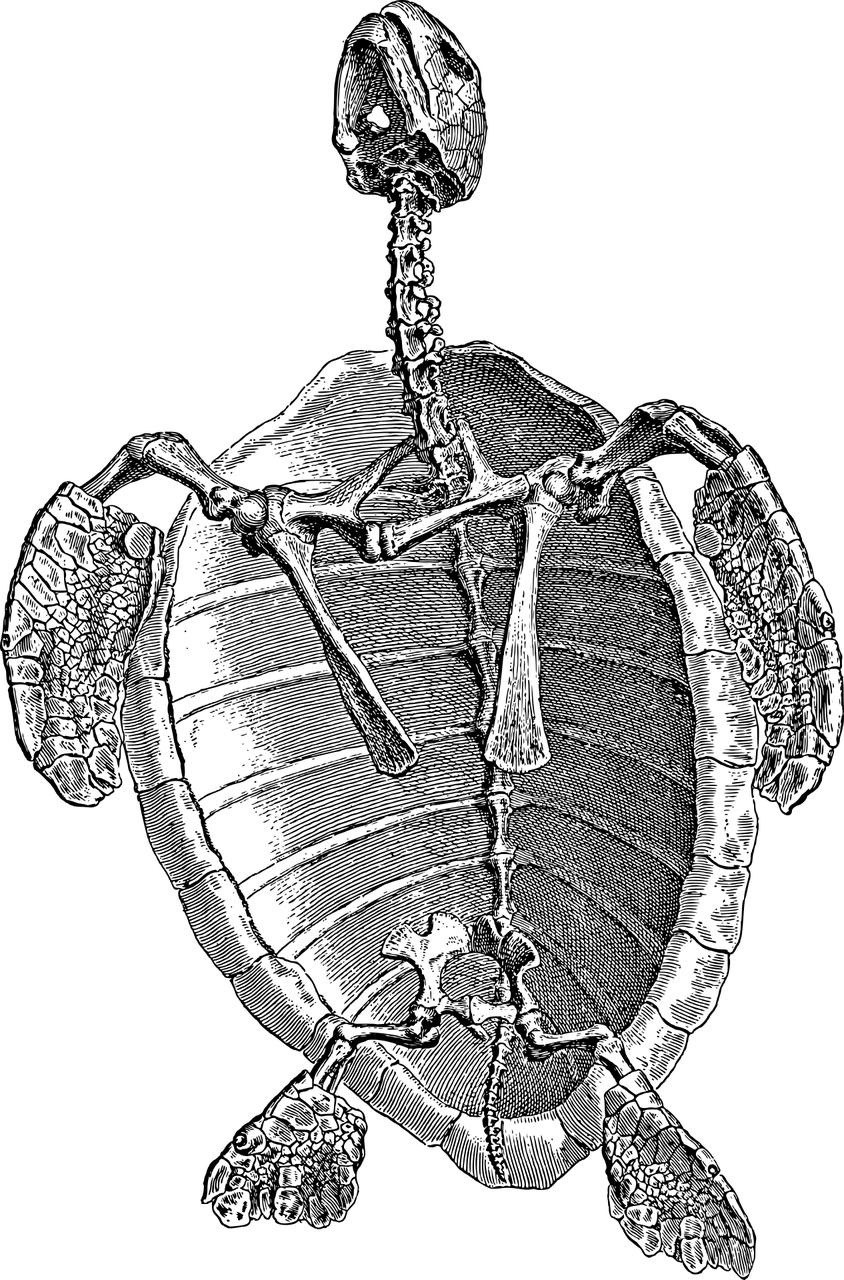
\includegraphics[
                    height=35mm,
                    width=\linewidth,
                    keepaspectratio
                ]{Relevancia/ecosistemas.png}
                \caption{Pérdida de biodiversidad}
            \end{figure}
        \end{column}
        \begin{column}{0.25\textwidth}
            \centering
            \begin{figure}
                \centering
                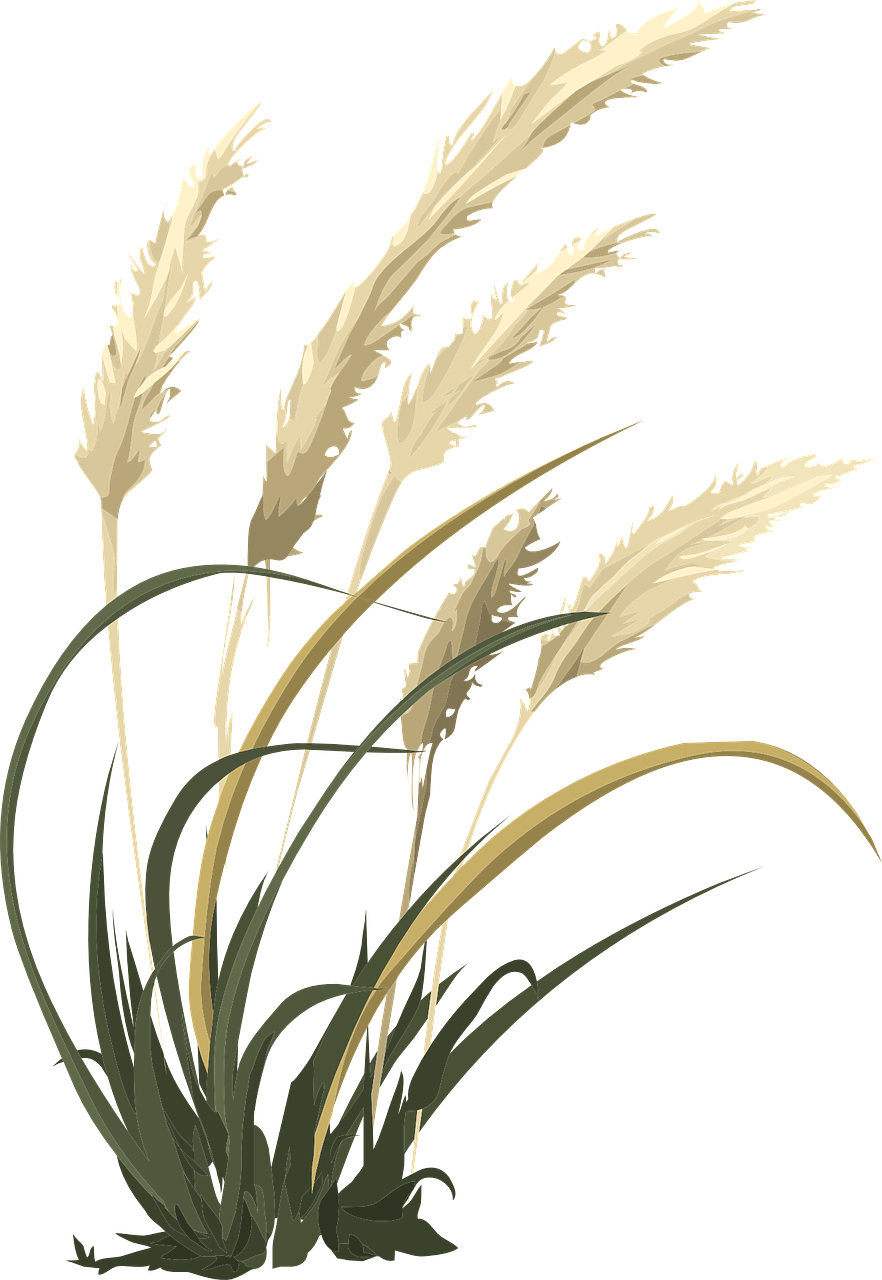
\includegraphics[
                    height=35mm,
                    width=\linewidth,
                    keepaspectratio
                ]{Relevancia/industrias.png}
                \caption{Afectaciones a industrias}
            \end{figure}
        \end{column}
        \begin{column}{0.25\textwidth}
            \centering
            \begin{figure}
                \centering
                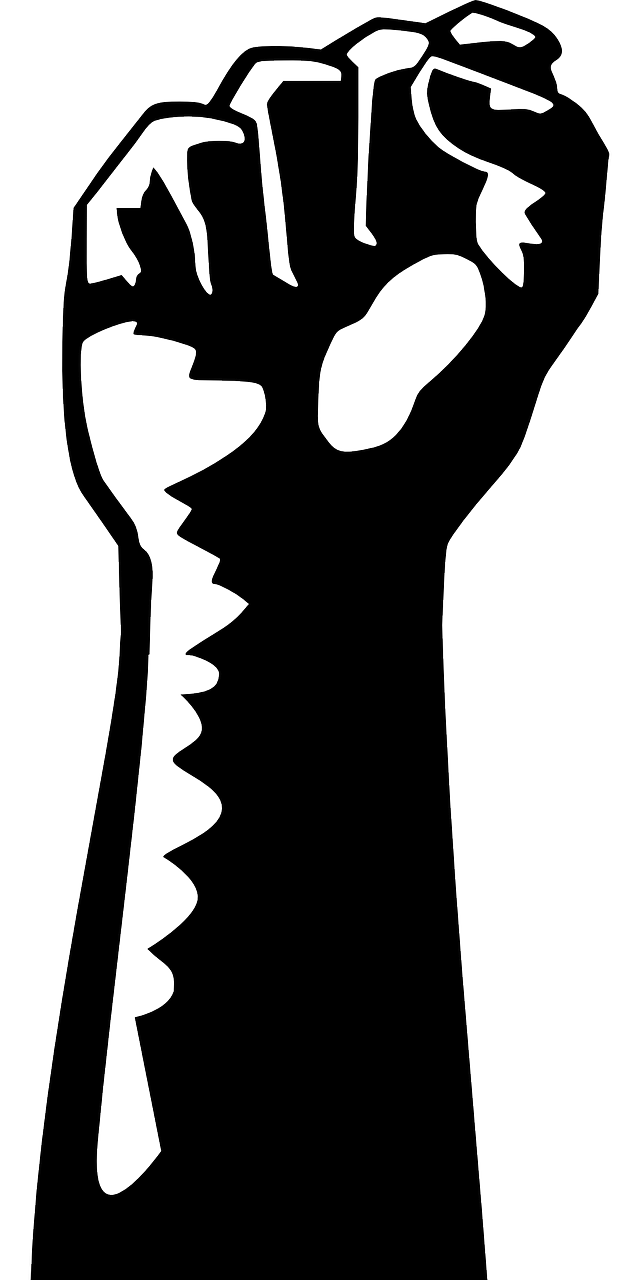
\includegraphics[
                    height=35mm,
                    width=\linewidth,
                    keepaspectratio
                ]{Relevancia/conflictos.png}
                \caption{Conflictos sociales}
            \end{figure}
        \end{column}
    \end{columns}
\end{frame}

\begin{frame}
    \frametitle{Planteamiento del problema}
    \begin{displayquote}
        \justifying
        \textbf{ODS 6.a.} De aquí a 2030, ampliar la cooperación internacional y el apoyo prestado a los países en desarrollo para la creación de capacidad en actividades y programas relativos al agua y el saneamiento, como los de captación de agua, \textbf{\gls{desalinizacion}}, uso eficiente de los recursos hídricos, tratamiento de aguas residuales, reciclado y tecnologías de reutilización \cite{naciones_unidas_sustainable_nodate}.
    \end{displayquote}\vspace*{6mm}
    \centering
    \begin{figure}
        \centering
        
\includegraphics[height=35mm, keepaspectratio]{ONU.png}
        
\includegraphics[height=35mm, keepaspectratio]{ods.png}
        \caption{Objetivos de desarrollo sostenible}
    \end{figure}
    
\end{frame}
	\input{Content/Justificación.tex}
	\section{Objetivos}

\begin{frame}[allowframebreaks]
    \frametitle{Objetivo General}
    \begin{center}
    		\Large\bfseries \centering Diseñar y construir un destilador solar activo usando concentradores solares de lentes de Fresnel para destilar agua salada.
    \end{center}
\end{frame}

\begin{frame}
    \frametitle{Etapa de diseño}
    
    \begin{enumerate}[I]
    		\item \textbf{Analizar los datos ambientales} de temperatura e irradiación solar \textbf{de la Ciudad de México} para tener información climática sobre el lugar donde se desarrollará el proyecto.
    		\item \textbf{Definir los parámetros asociados} a la desalinización con los que operará el sistema tales como la taza volumétrica de agua o la salinidad del agua de alimentación.
        \item \textbf{Diseñar los sistemas de tuberías} y almacenamiento donde fluirá y reposará el agua salada.
        \item \textbf{Diseñar el concentrador solar} y el mecanismo con el que se integrará al sistema de tuberías.
        \item \textbf{Estudiar los modelos térmicos} que caractericen o aproximen el comportamiento del concentrador solar y del proceso de evaporación.
    \end{enumerate}
\end{frame}

\begin{frame}
	\frametitle{Etapa de construcción}
	
	\begin{enumerate}[I]
		\item Construir los componentes que integran al destilador solar con base en los diseños propuestos.
		\item Desarrollar el \textbf{mecanismo de control} para regular la velocidad de flujo del agua mediante la implementación de programación y sistemas de control.
		\item \textbf{Integrar a un seguidor solar} el concentrador para mejorar la captación de calor.
		\item \textbf{Evaluar el desempeño} del destilador solar con base en el agua de salida para verificar la viabilidad del mismo.
	\end{enumerate}
\end{frame}	
	\section{Antecedentes}

\begin{frame}
	\frametitle{Desalinizador autónomo}
	En 2018 se desarrolló un destilador solar activo e híbrido, capaz de destilar hasta \SI{10}{\litre} por día en días soleados usando precalentamiento de agua\\
	\begin{figure}
		\centering
		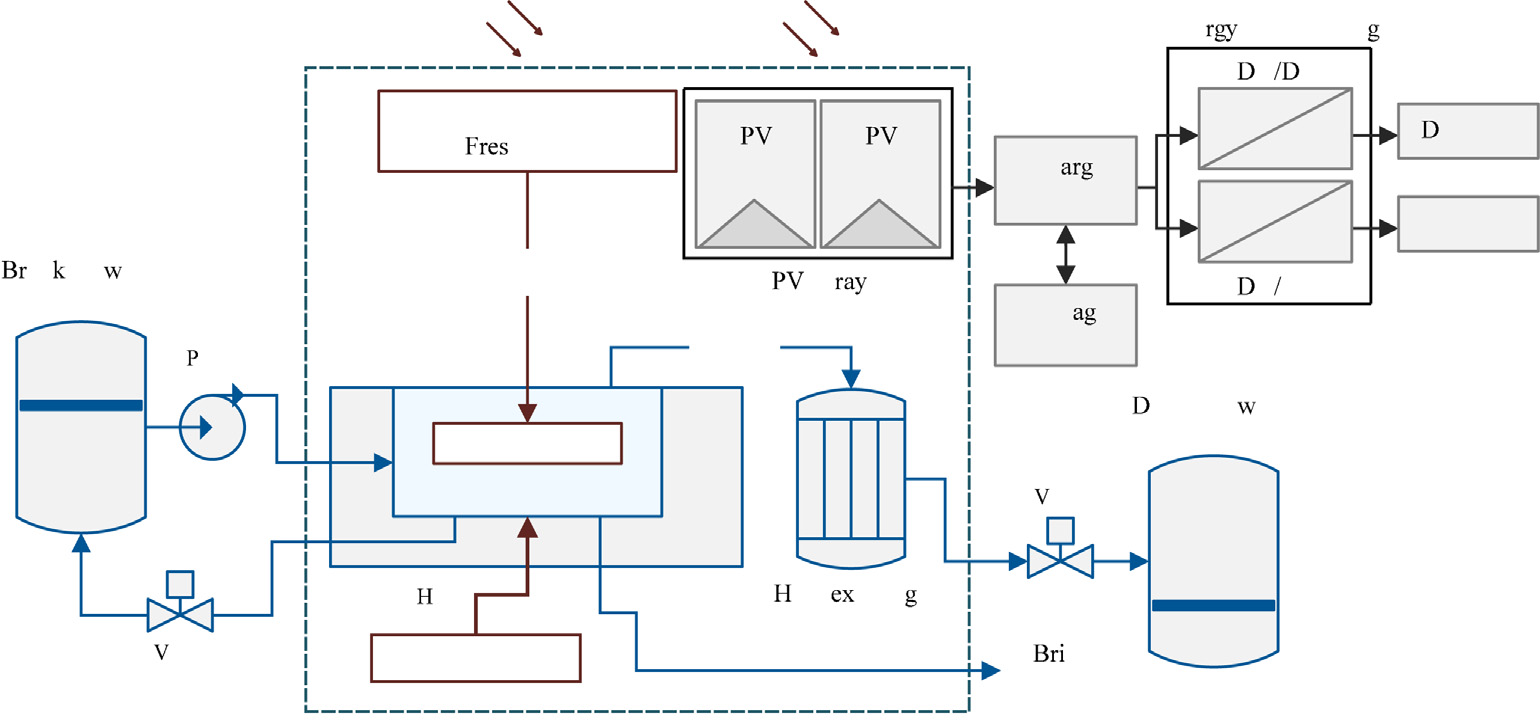
\includegraphics[
			height=45mm,
			width=\linewidth,
			keepaspectratio
		]{destilador-palomino.png}
		\caption{Destilador solar activo de Palomino et. al}
		{\scriptsize\fullcite{palomino-resendiz_design_2018}}
	\end{figure}
\end{frame}


\begin{frame}
	\frametitle{Desalinizador de doble cámara}
	En 2022 se desarrolló un destilador solar activo el cual tuvo una producción de \qty{4.03}{\litre\per\metre\tothe{2}} por día.\\
	\begin{figure}
		\centering
		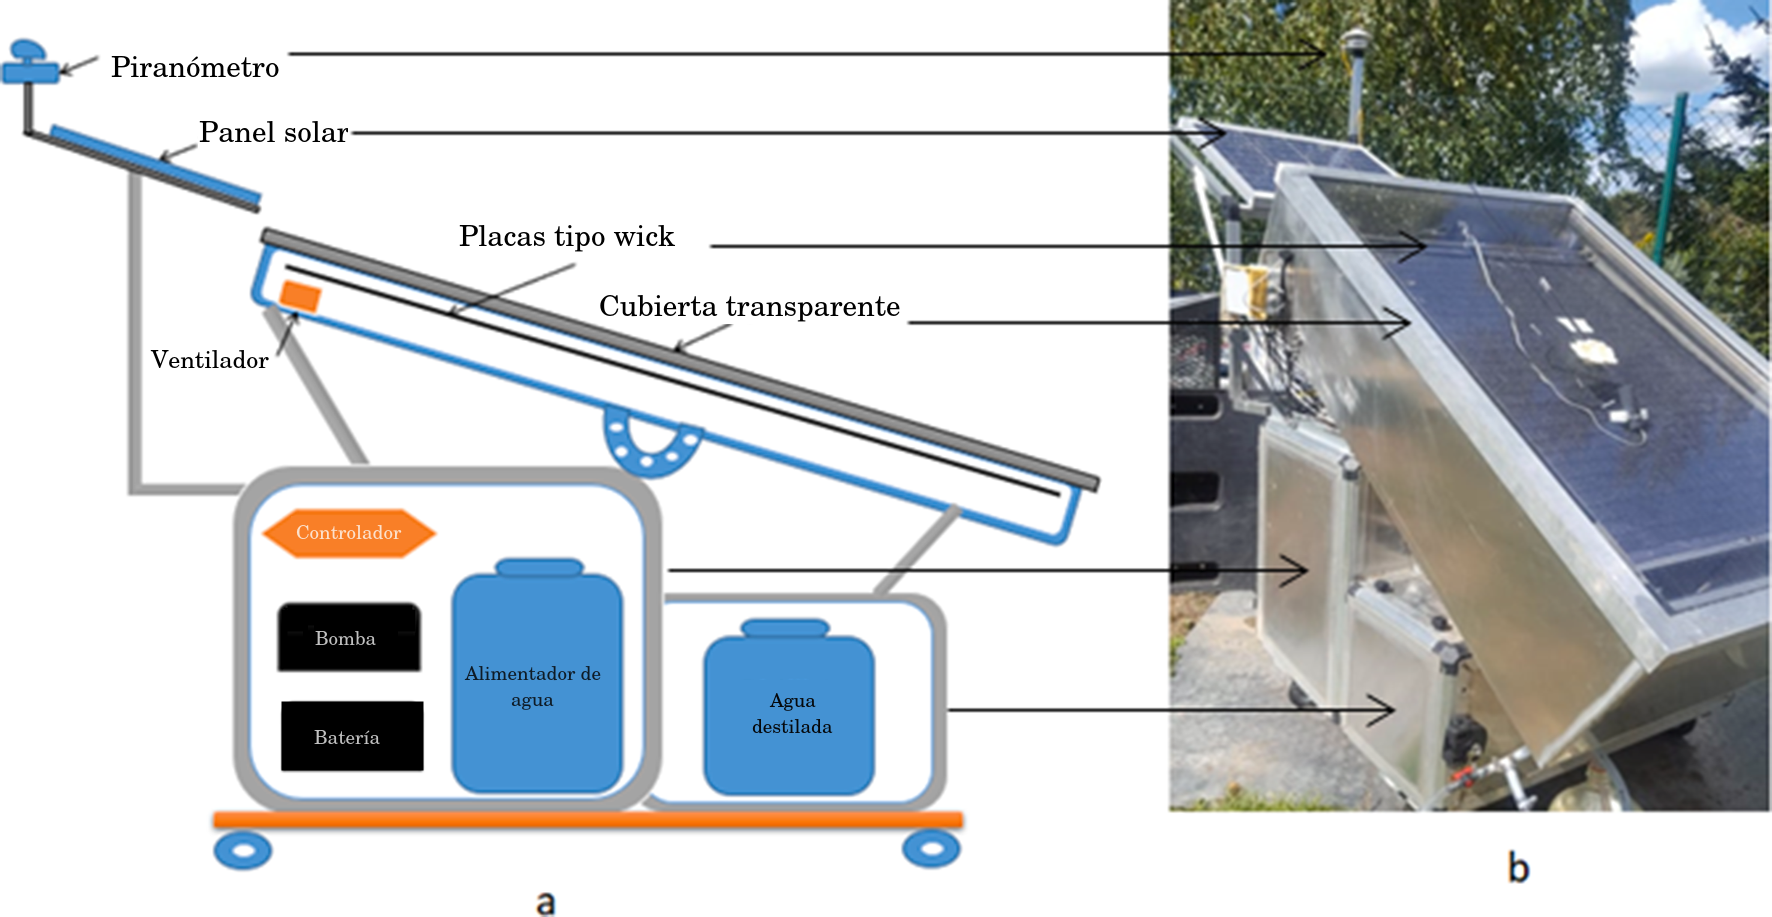
\includegraphics[
			height=45mm,
			width=\linewidth,
			keepaspectratio
		]{solar-wick-distiller.png}
		\caption{Destilador solar de doble cámara}
		{\scriptsize\fullcite{jobrane_theoretical_2022}}
	\end{figure}
\end{frame}
	\input{Content/Marco-teórico.tex}
	\input{Content/Diseño-experimental.tex}
	\section{Resultados}

\begin{frame}
	\frametitle{Desalinizador propuesto}
	Se propone un desalinizador de 4 cámaras integradas verticalmente\\
	\begin{figure}
		\centering
		\only<1>{
		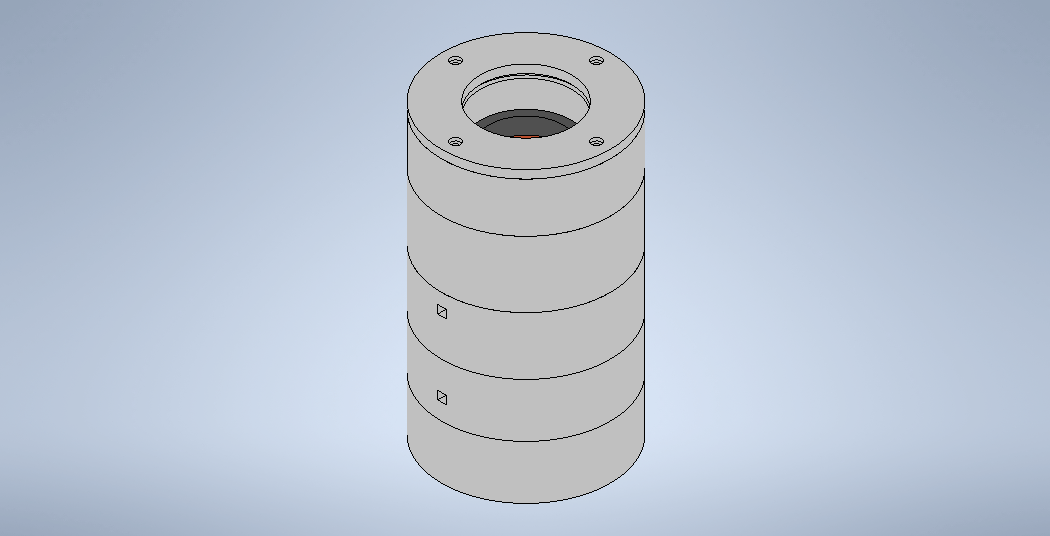
\includegraphics[
			height=60mm,
			width=\linewidth,
			keepaspectratio
		]{Resultados/Sistema/Desalinizador.png}
		}
		\only<2>{
		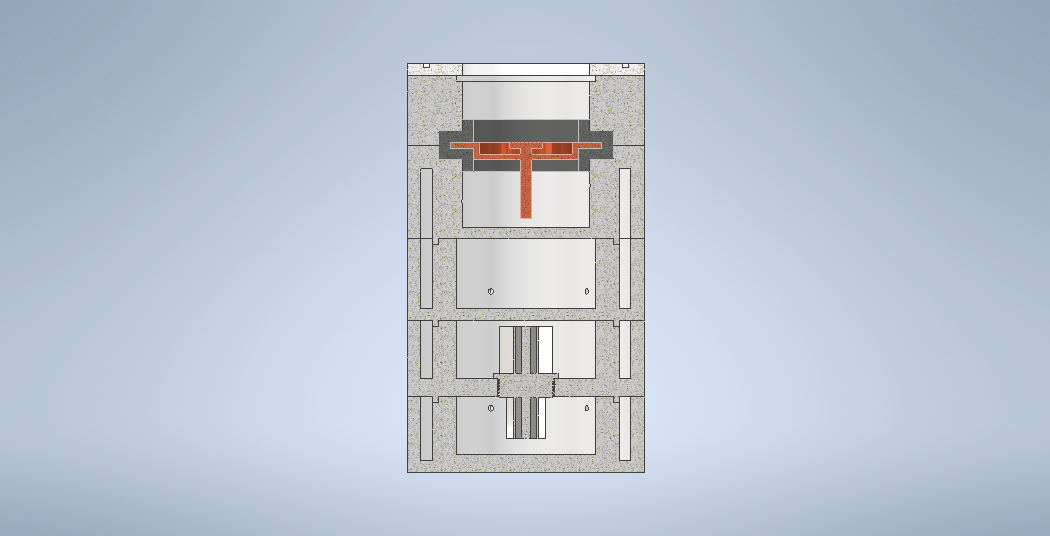
\includegraphics[
			height=60mm,
			width=\linewidth,
			keepaspectratio
		]{Resultados/Sistema/corte-desalinizador.png}
		}
		\caption{Desalinizador propuesto}
	\end{figure}
\end{frame}

\begin{frame}
	\frametitle{Contenedor de agua de mar}
	
	\begin{figure}
		\centering
		\only<1>{
		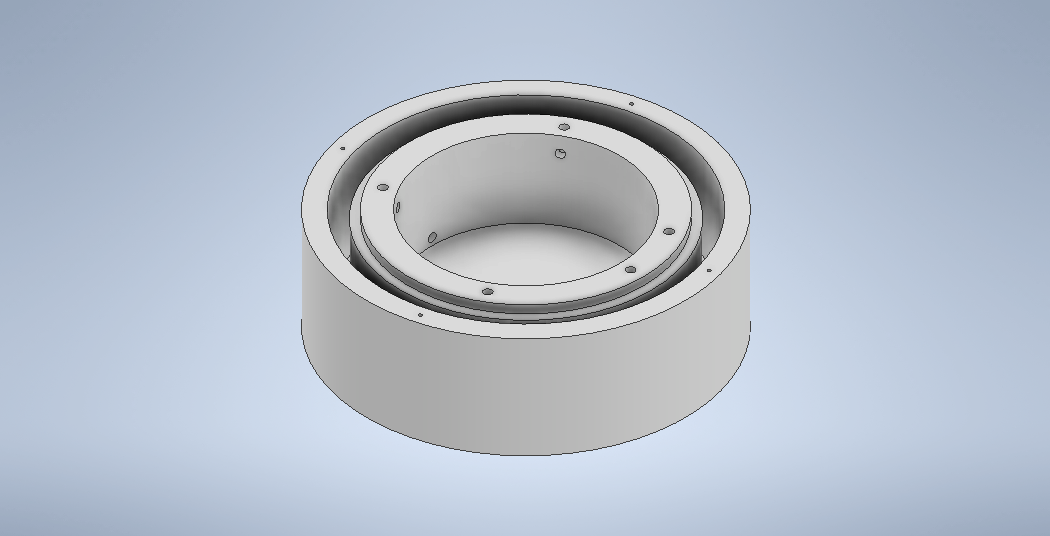
\includegraphics[
			height=45mm,
			width=\linewidth,
			keepaspectratio
		]{Resultados/Cortes/Contenedor-agua-mar.png}
		}
		\only<2>{
		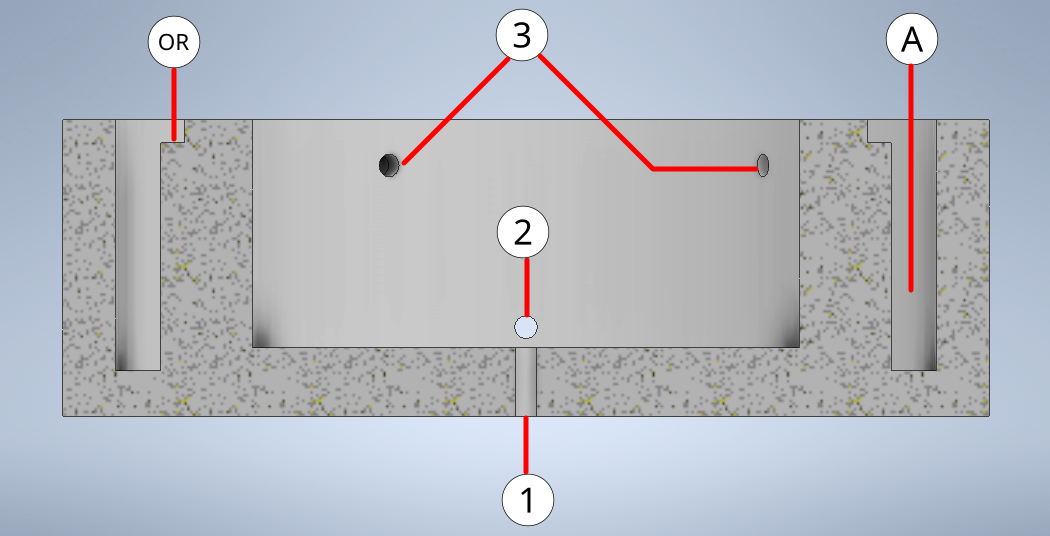
\includegraphics[
			height=45mm,
			width=\linewidth,
			keepaspectratio
		]{Resultados/Cortes/Contenedor-agua-mar-corte-1.png}
		}
		\only<3>{
		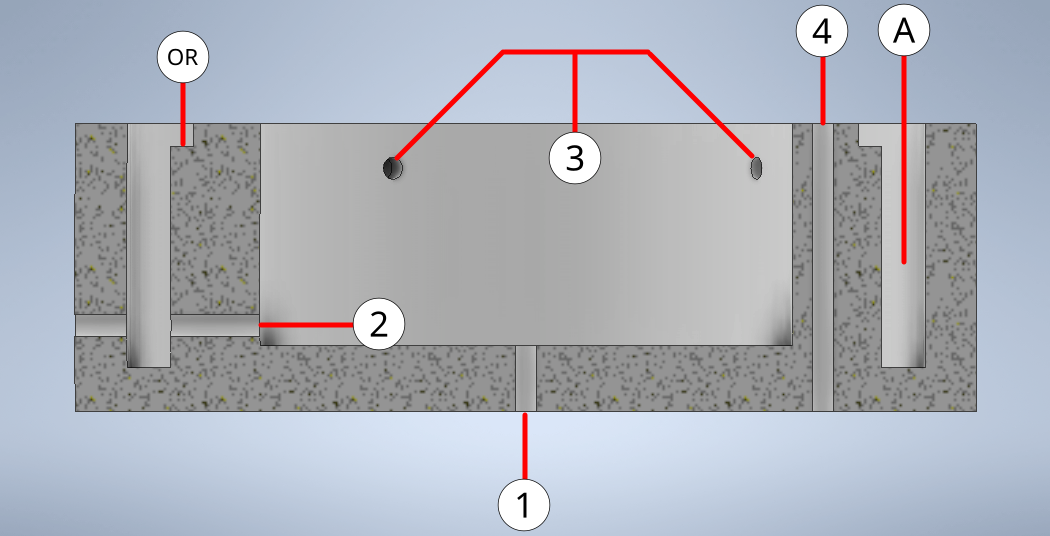
\includegraphics[
			height=45mm,
			width=\linewidth,
			keepaspectratio
		]{Resultados/Cortes/Contenedor-agua-mar-corte-2.png}
		}
		\caption{Contenedor de agua de mar}
	\end{figure}
	
	1) Salida a bomba. 2) Entrada agua. 3) Retroalimentación. 4) Bombeo agua.\\
	OR) Sellado. A) Aislante
	
\end{frame}

\begin{frame}
	\frametitle{Cámara de condensación}
	
	\begin{figure}
		\centering
		\only<1>{
		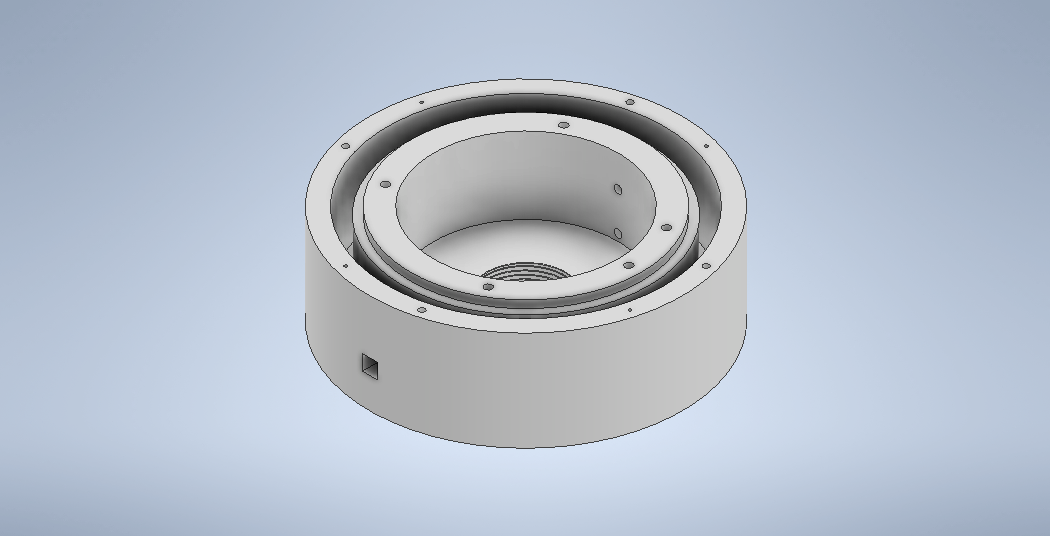
\includegraphics[
			height=45mm,
			width=\linewidth,
			keepaspectratio
		]{Resultados/Cortes/Contenedor-agua-destilada.png}
		}
		\only<2>{
		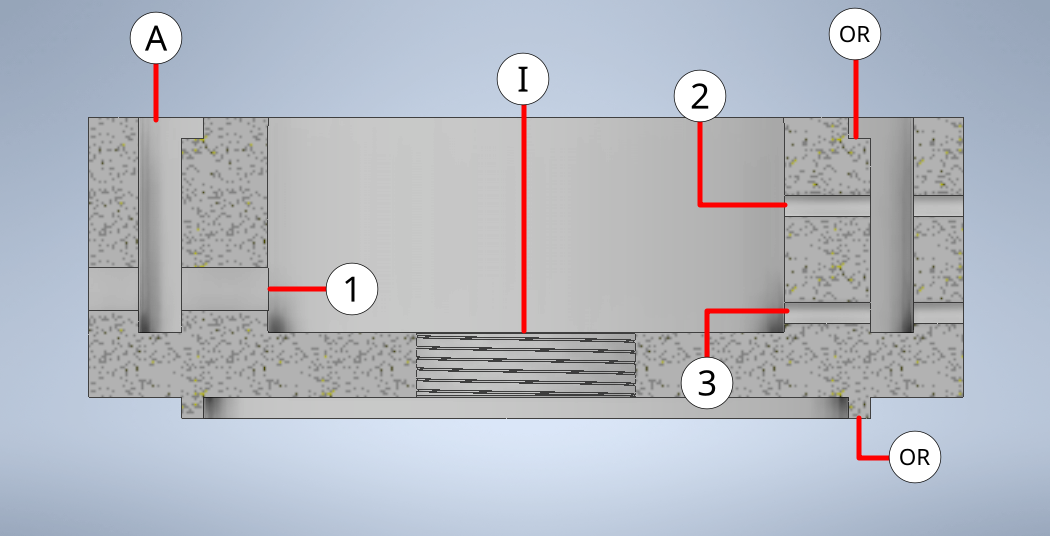
\includegraphics[
			height=45mm,
			width=\linewidth,
			keepaspectratio
		]{Resultados/Cortes/Contenedor-agua-destilada-corte-1.png}
		}
		\only<3>{
		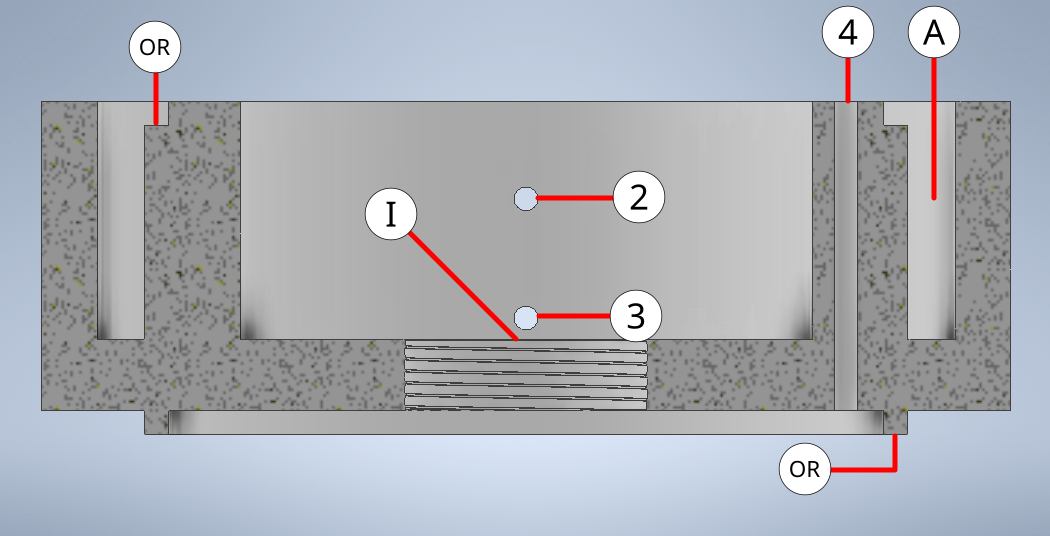
\includegraphics[
			height=45mm,
			width=\linewidth,
			keepaspectratio
		]{Resultados/Cortes/Contenedor-agua-destilada-corte-2.png}
		}
		\caption{Cámara de condensación}
	\end{figure}
	
	1) Entrada vapor. 2) Salida salmuera. 3) Salida agua destilada. 4) Bombeo agua.\\
	
	OR) Sellado. A) Aislante. I) Intercambiador
	
\end{frame}

\begin{frame}
	\frametitle{Intercambiador de calor}
	
	\begin{figure}
		\centering
		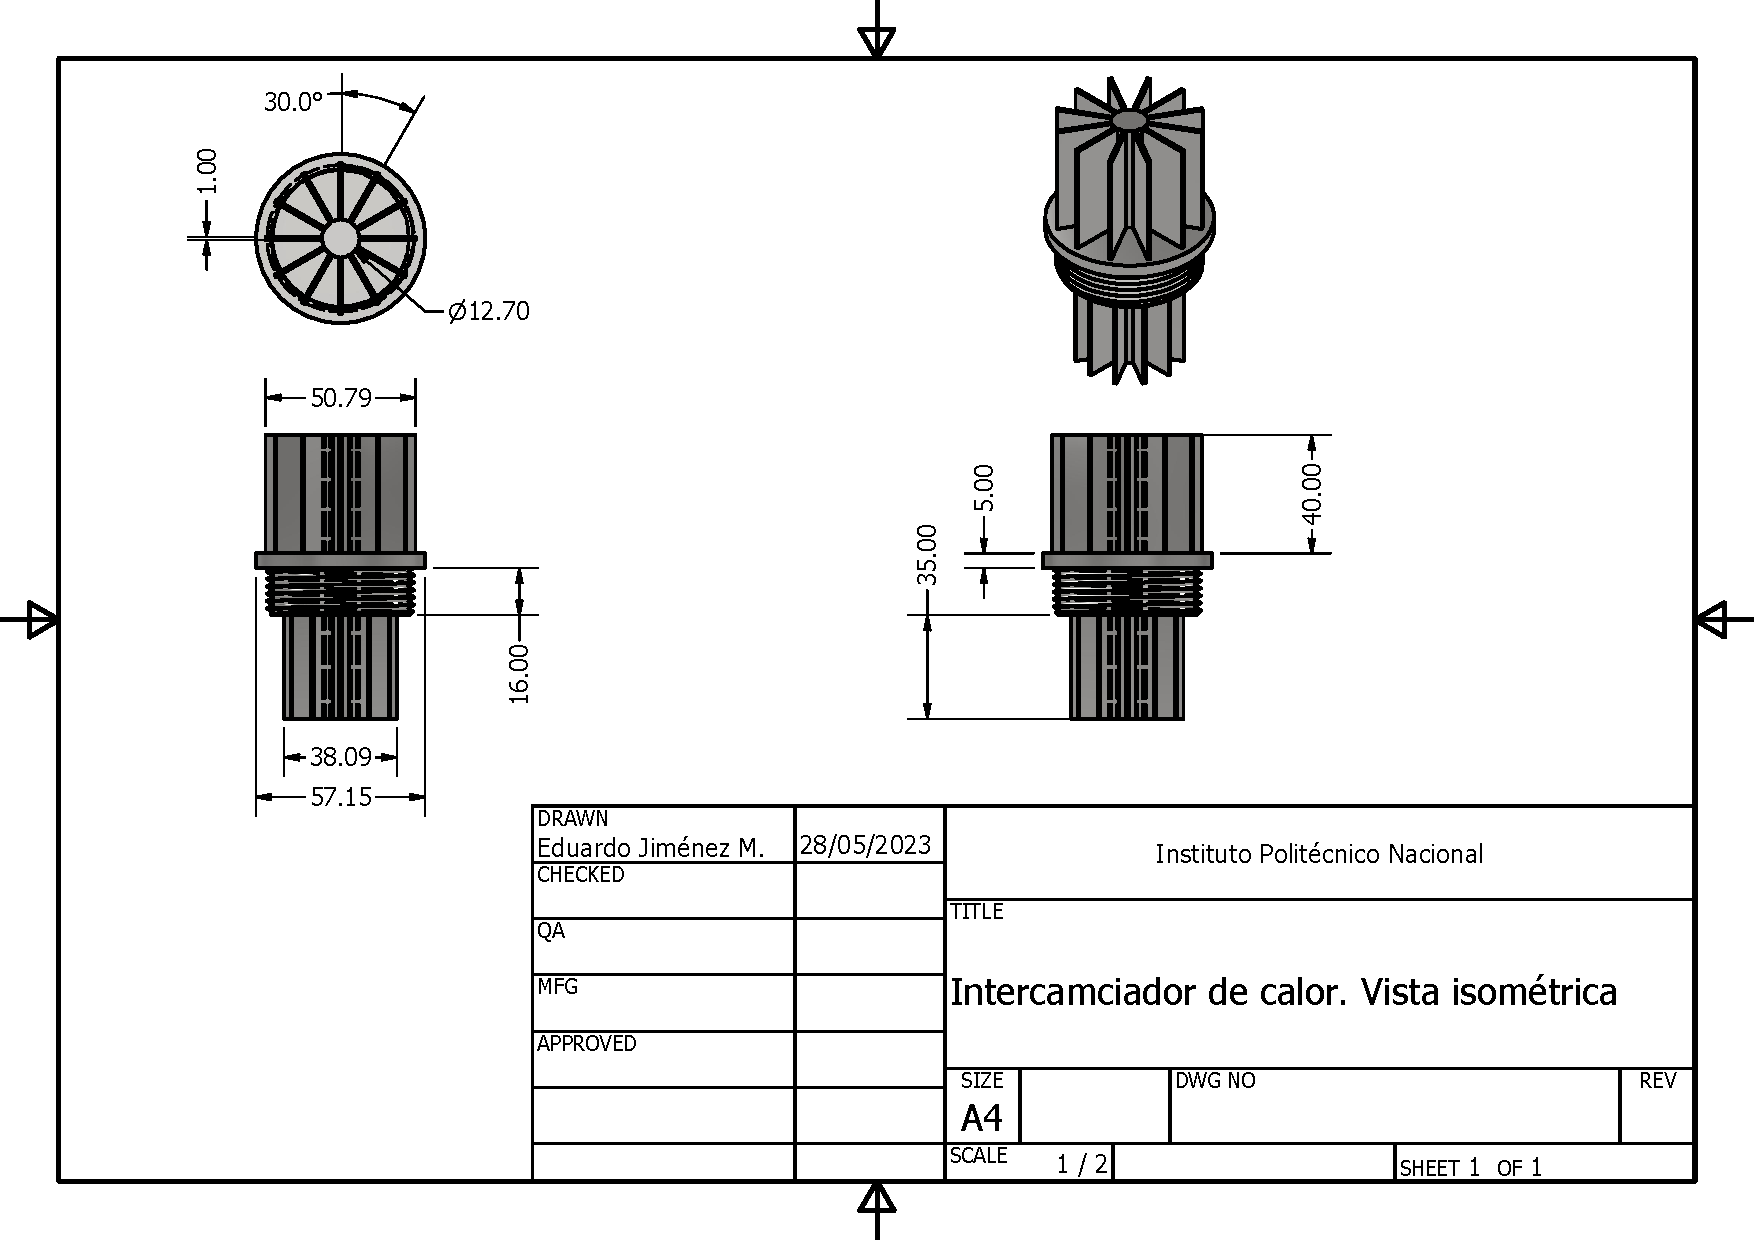
\includegraphics[
			height=75mm,
			width=\linewidth,
			keepaspectratio
		]{Resultados/Sistema/intercambiador.pdf}
		\caption{Intercambiador de acero 316}
	\end{figure}
	
\end{frame}

\begin{frame}
	\frametitle{Cámara de evaporación}
	
	\begin{figure}
		\centering
		\only<1>{
		\includegraphics[
			height=45mm,
			width=\linewidth,
			keepaspectratio
		]{Resultados/Cortes/camara-evaporación.png}
		}
		\only<2>{
		\includegraphics[
			height=45mm,
			width=\linewidth,
			keepaspectratio
		]{Resultados/Cortes/camara-evaporación-corte-1.png}
		}
		\only<3>{
		\includegraphics[
			height=45mm,
			width=\linewidth,
			keepaspectratio
		]{Resultados/Cortes/camara-evaporación-corte-2.png}
		}
		\caption{Cámara de condensación}
	\end{figure}
	
	1) Salida vapor. 2) Salida salmuera. 3) Desagüe. 4) Bombeo agua.\\
	
	OR) Sellado. A) Aislante
	
\end{frame}

\begin{frame}
	\frametitle{Cámara de transferencia parte inferior}
	
	\begin{figure}
		\centering
		\only<1>{
		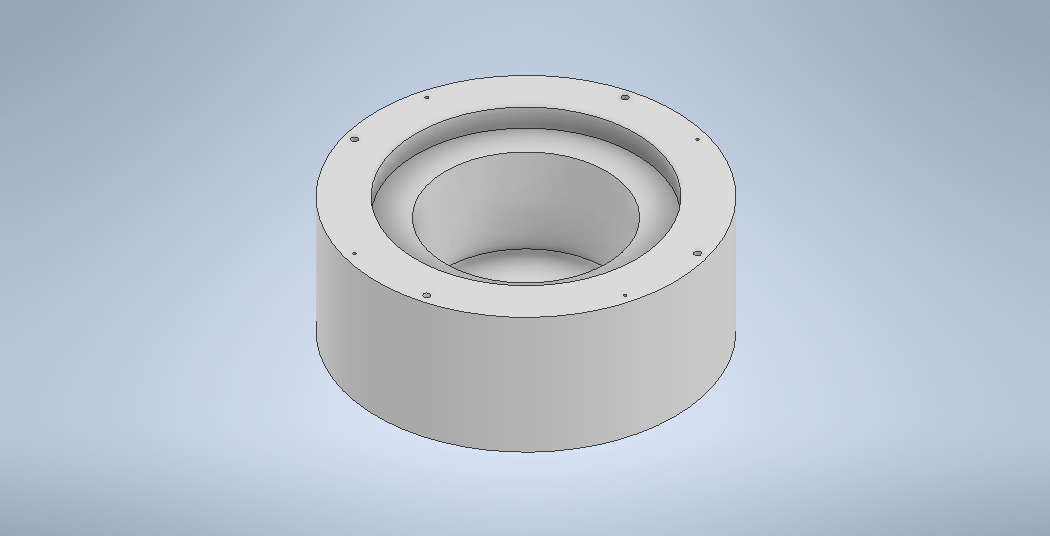
\includegraphics[
			height=45mm,
			width=\linewidth,
			keepaspectratio
		]{Resultados/Cortes/Arena-concentrador.png}
		}
		\only<2>{
		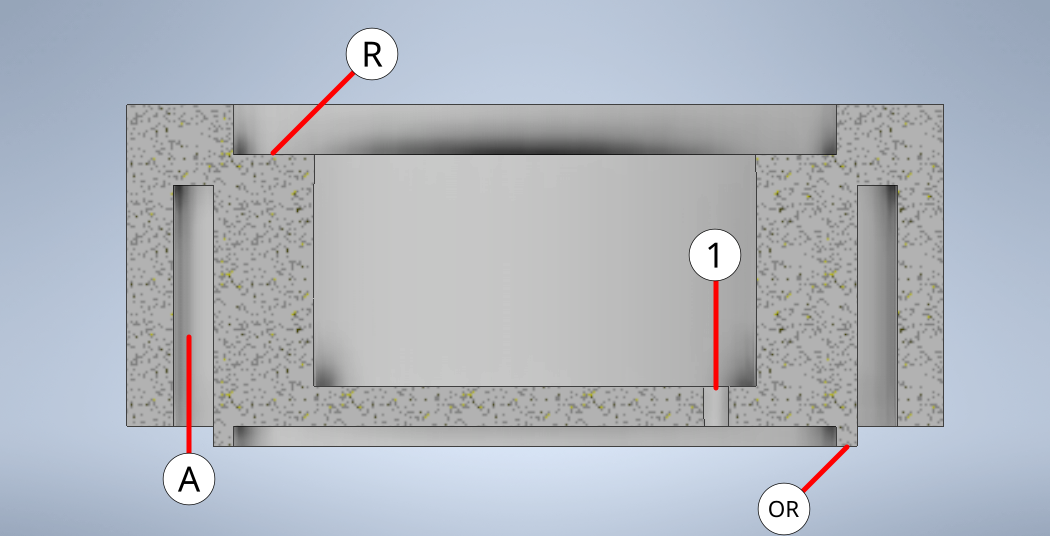
\includegraphics[
			height=45mm,
			width=\linewidth,
			keepaspectratio
		]{Resultados/Cortes/Arena-concentrador-corte-1.png}
		}
		\only<3>{
		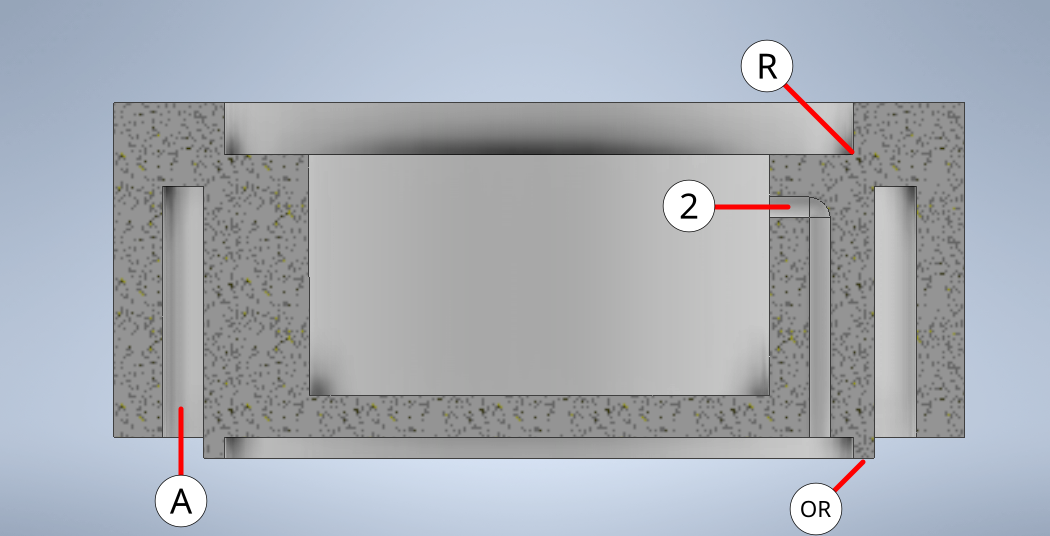
\includegraphics[
			height=45mm,
			width=\linewidth,
			keepaspectratio
		]{Resultados/Cortes/Arena-concentrador-corte-2.png}
		}
		\caption{Cámara de transferencia parte inferior}
	\end{figure}
	
	1) Salida agua caliente. 2) Entrada agua fría \\
	
	OR) Sellado. A) Aislante. R) Recibidor
	
\end{frame}

\begin{frame}
	\frametitle{Cámara de transferencia parte superior}
	
	\begin{figure}
		\centering
		\only<1>{
		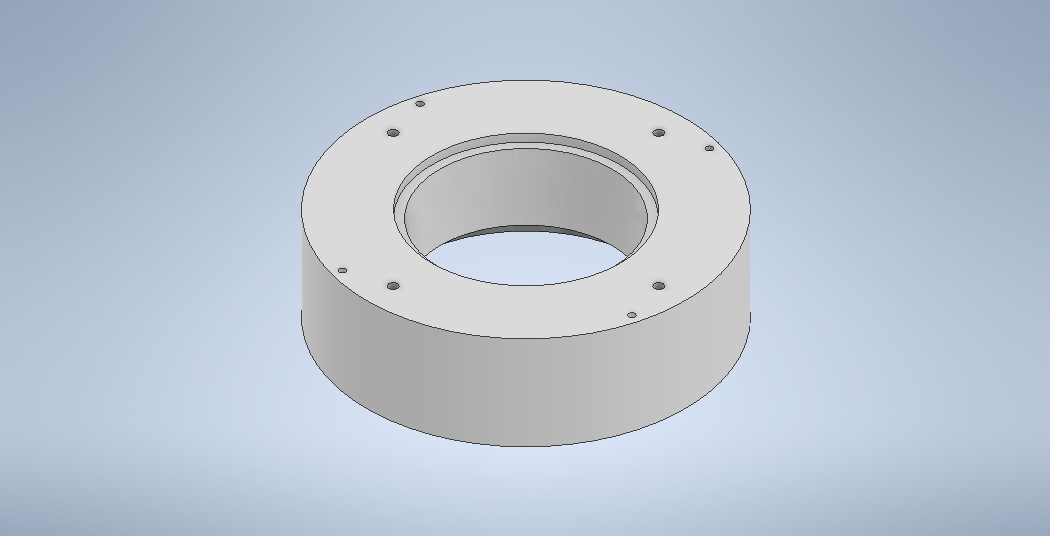
\includegraphics[
			height=45mm,
			width=\linewidth,
			keepaspectratio
		]{Resultados/Cortes/Concentrador.png}
		}
		\only<2>{
		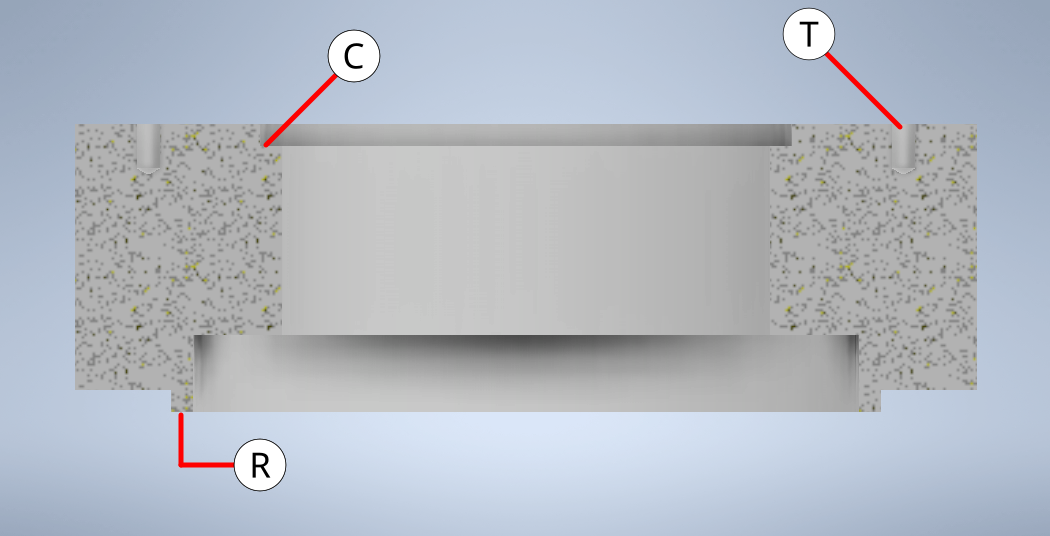
\includegraphics[
			height=45mm,
			width=\linewidth,
			keepaspectratio
		]{Resultados/Cortes/Concentrador-corte-1.png}
		}
		\caption{Cámara de transferencia parte superior}
	\end{figure}
	
	C) Cuarzo. R) Recibidor. T) Tornillo
	
\end{frame}

\begin{frame}
	\frametitle{Recibidor solar}
	
	\begin{figure}
		\centering
		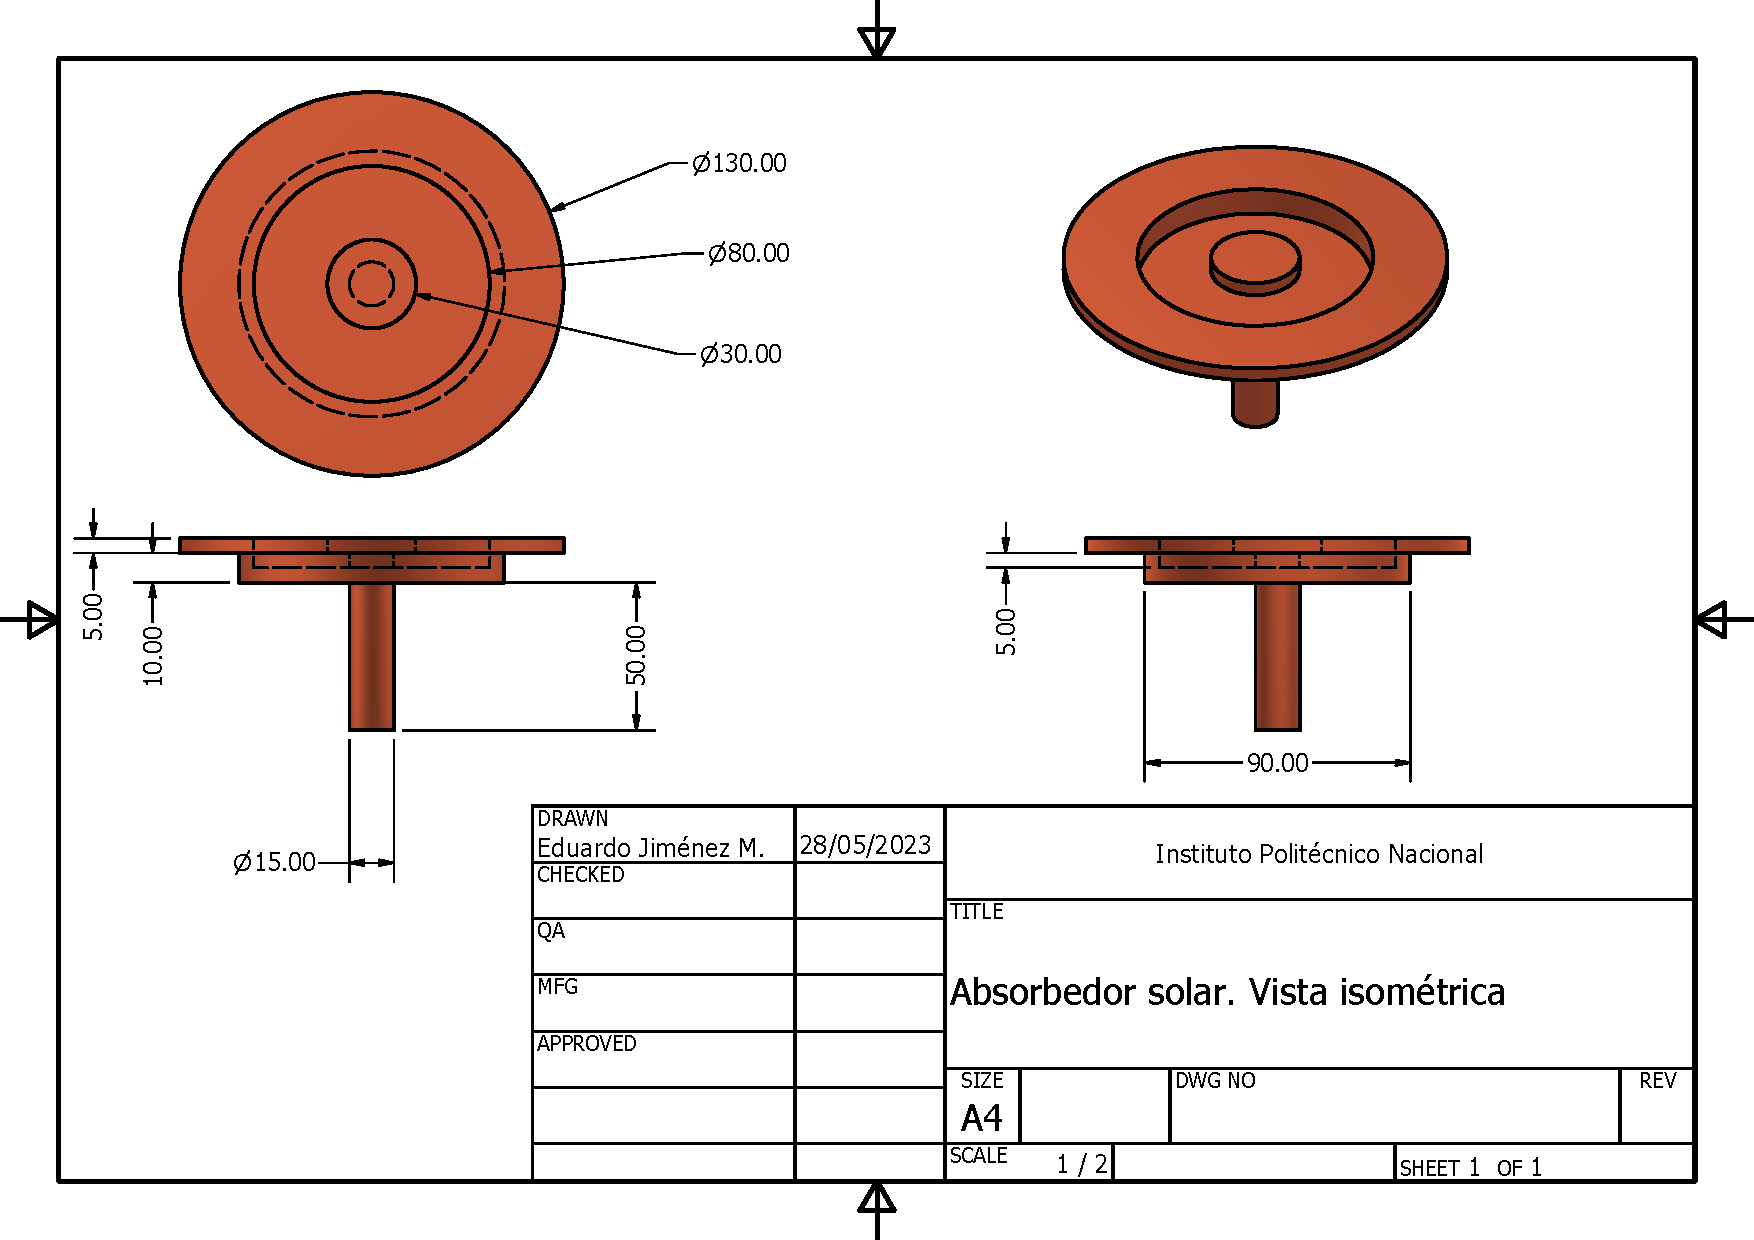
\includegraphics[
			height=70mm,
			width=\linewidth,
			keepaspectratio
		]{Resultados/Sistema/absorbedor.pdf}
		\caption{Recibidor solar}
	\end{figure}
	
\end{frame}
	\input{Content/Recapitulación.tex}
	
	\begin{frame}[allowframebreaks]
		\frametitle{Referencias}
		\printbibliography
	\end{frame}
	
\end{document}
